\documentclass[11pt,twocolumn]{article}
\usepackage[left=1in,top=1in,right=1in,bottom=1in,nohead,foot=1cm]{geometry} 
\usepackage{aaai}
\usepackage{times}
\usepackage{tikz}
\usepackage{pgfplots}
\usepackage{amsmath,amssymb}
\usepackage{graphicx,psfrag}
\usepackage{amsthm} 
\usepackage{setspace}
\usepackage{comment}
\usepackage{algorithm}
\usepackage{algorithmic}
\DeclareMathSymbol{\R}{\mathbin}{AMSb}{"52}

%\doublespacing

\newtheorem{lemma}{Lemma}
\newtheorem{theorem}{Theorem}

\title{GiftGiver: The Gift Recommender \\ {\small AAI --
    Instructor: Prof. Jane Hsu}}
\author{Weiti Kuo, Penn Su, George Chang \\ \{r99922003, r99922157, r99944002\}@csie.ntu.edu.tw}
\begin{document}
\maketitle

\section{Introduction}

Although picking gifts for your best friend or your beloved family member are so common in daily life, often people had been troubled by it. People had been overwhelmed by the number of choices given by the commercial retailer stores and e-commerce websites, however, most of the gift recommendation websites aren't good enough for the general public because most of the gifts were cliche or repetitive there are also no common sense in those recommendation websites.

There are many factors to affect final decision. As a sender, budget is a big issue. Even the sender spends a lot of money preparing a gift, the receiver may think it too expensive and embarrassed to receive it.   Under tight budget, sender might consider the receiver's interest, religious, gender, age, and the relationship between the receiver and you. In addition, the date to gift is also a very important factor. Under normal circumstances, you do not send a coat in a hot summer.

How to find a suitable gift? In the past, you go to a department store, and try to find the ideal gift, browsing through one store after the other, but nothing seems perfect. If you are not a decisive one, the process is time-consuming. At present, there are many online website to recommend gifts, e.g. Gift ideas, Hallmark Cards, Amazon gifts, Find gift, Yahoo! Gift Finder, JCpenny, Macy's, Sears[Reference]. However, according to our observations, most of them cannot supply satisfactory service. Usually, gifts websites prefer using best seller to be their recommendations. The gift website usually comes out the similar recommendation list event we sent the different preferences, occasion and receiver’s age, and the list has too many details.

Some people ask others' opinions when they are picking a nice gift, but gift giving should kept secret to the receiver, the gift might not be a surprise when everyone knows about it.

Based on the above reasons, we explored a system we called "GiftGiver" to recommend a list of gifts to help senders. In order to figure out what should be a nice gift,  we followed the idea of Scenario-Oriented Recommendation~\cite{Shen}.   We analyzed each gift into 8 features. GiftGiver come out a concept of the gift idea, such like flower, tea mug etc.  In the way that sender can have their own gift choice.  If sender has no idea about a particular item, our system can also gives sender the detail of the gift given from other e-commerce websites.

To give more variety of the recommendations for different occasions and different personalities, we built a website.   The UI content includes occasion, relationship, sender's favor, receiver's profile. 
Sender can easily fill in their consideration step by step. 
After fill in the answer, system will comes out 20 recommended gifts.  If receiver are not satisfied, he/she can also change the answer and search again.

We tried to make a system to be a good helper for the people who might just want a general nudge to the right directions or some inspirations on what to sent.  

\section{Related Work}
Traditionally, recommender systems are classified into the following three categories: 
1. User-based Collaborative Filtering Systems~\cite{Herlocker}:
The user will be recommended items similar to the ones the user preferred in the past.
2. Item-based Collaborative Filtering Systems~\cite{Sarwar, Linden}:
The user will be recommended items that people with similar tastes and preferences liked in the past.
3. Hybrid Recommender Systems[Reference 2篇]:
These methods combine the above two methods.
They usually suggest books, music albums, from a set of input parameters, possibly including user profiles, purchase history, etc.

In recent years, many researchers use novel technology to recommend, e.g. Edward use Commonsense to recommend clothing [ ].   Furthermore, some researchers use recommender system in interesting domains, such as Cosley’s Movie Recommendation[ ], and Koutrika’s Course Recommendation[ ].   Moreover, the display style of Top 10 is popular again recently []. We follow the latest trend, and use the novel technology in interesting domain.   In short, we are the first one that combine traditional recommendations and Commonsense, and apply them in Gift Recommendation.


\section{System Architecture}

This section describes the basic structure of our system, the flow of the system and we go through some of the UI designs and finally touch on the algorithms we used to rank and filter the gift list.

\subsection{Flow}
Users of our recommender system start with filling in their considerations on the UI interface. (For reducing the loading of senders, we use check box and combo box and make a lot of common options.)   
After filling in the options and considerations, the users will be greeted  a list of 20 recommended gifts generated by the system from the information provided by the users.
If the users want more information on the recommended gift item, they can click the link and the system will help the users to find the relative products from several popular e-commerce websites.

\begin{figure}[h!t]
\centering{
    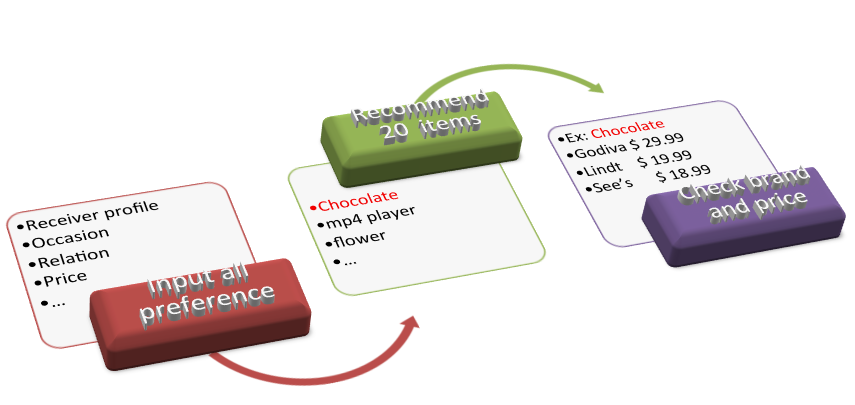
\includegraphics[width=\linewidth]{flow.png}
}
\caption{Flow Chart}
\end{figure}


\subsection{UI Design}
The UI of the GiftGiver is given in Figure~\ref{ui}, it is a website with a rich set of options for users to choose his/her preference for the gifts. We categorize the questions in to 3 main parts, the main considerations, the Receiver profile and the Result based on the result of the questionnaire. Originally we considered both the features and preference of the sender and the receiver, however we want to learn more about what might be the influencial factors for picking gifts.  We designed a questionnaire to ask 3 adult females and 10 adult males about what they will consider when they sent a gift.
(The question is like “when you are picking a gift, is the relation between you and receiver seems important to you?”)   Each question has a scale from 1 to 5, from unimportant to most important.

(From the result table, we can separate the score in to 3 part – Red (score> 4), pink (4>score>3), and green (3>score).  The red part is the most important union.  Such as relationship, price, sender’s gender etc. This result is quiet reasonable.   In general, the gift will finally own by the receiver than own by both sender and receiver.   So the options about receivers are higher than the options about senders.  In other part, price, occasion, sent date and receiver’s gender are common to affect whether the gift is reasonable.)

Furthermore, we interviewed 5 differnet people with the primary concerns when picking a nice gift. We later found out the result of the interviews that they agreeed the same considerations with the questionnaire results. The results had shown that people  concern about the occasion more than relationship.  Other considerations did not seem to influence too much to the decision making process compared to occasion and relationship.

Based on those two results from two different groups of people, we cut off some of the considerations from original design, such as Sender's religion, Sender's Gender, etc.


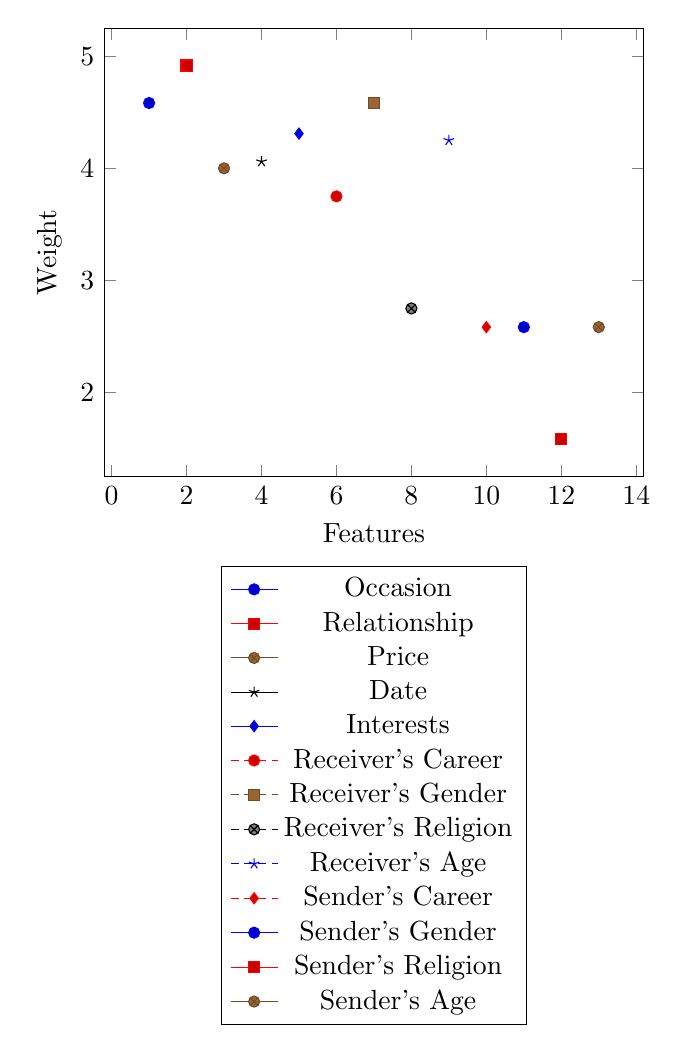
\begin{tikzpicture}
    \begin{axis}[xlabel=Features, ylabel=Weight, legend style={at={(0.5, -0.2)}, anchor=north}]
    \addplot coordinates {(1, 4.583)};
    \addplot coordinates {(2, 4.917)};
    \addplot coordinates {(3, 4)};
    \addplot coordinates {(4, 4.06)};
    \addplot coordinates {(5, 4.31)};
    \addplot coordinates {(6, 3.75)};
    \addplot coordinates {(7, 4.583)};
    \addplot coordinates {(8, 2.75)};
    \addplot coordinates {(9, 4.25)};
    \addplot coordinates {(10, 2.583)};
    \addplot coordinates {(11, 2.583)};
    \addplot coordinates {(12, 1.583)};
    \addplot coordinates {(13, 2.583)};
    \legend{Occasion,Relationship,Price,Date,Interests,Receiver's Career,Receiver's Gender,Receiver's Religion,Receiver's Age,Sender's Career,Sender's Gender,Sender's Religion, Sender's Age}
    \end{axis}
\end{tikzpicture}


Compare to major e-commerce websites that sells real products, our website doesn't have the real database for all different kinds of gifts, but we had a better flow and more variety and flexibility of options for users to pick. There is also another extinction between our UI design and those of major corporations. For example, Gifts.com has 9 ages degree, such as [0-6], [7-12], [13-19], [20-30], [31-40] etc, we use fuzzy set to define our age instead of clear separation by years. Because nouns like child, adult etc. will help the system in the commonsense part.  On the other hand, some people still looks like a child even that person has already more than 30s.  The fuzzy part will come out positive result.




\begin{figure}[h!t]
\centering{
    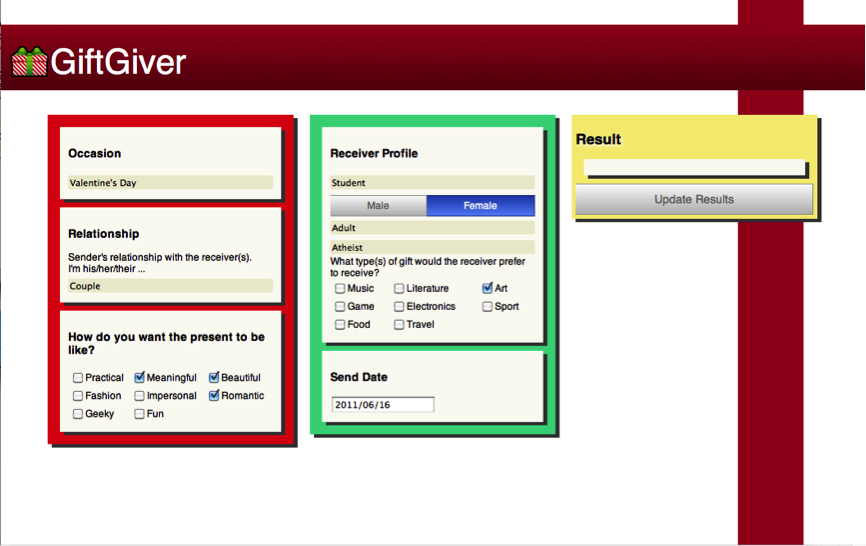
\includegraphics[width=\linewidth]{ui.png}
}
\caption{UI design}
\label{ui}
\end{figure}

\subsection{Methodology}

This section briefly discussed our appoaches to rank the gifts and algorithms with commonsense knowledge base

\subsubsection{Feature Vectors}

We have decided to take a feature matching approach of the recommendation system.
We analyze 60 gifts items and 3 common occasions and extract only 8 features.  
The features are listed in Table~\ref{features}.


\begin{table*}[ht]
\caption{Feature Vector}
\centering
\begin{tabular}{l l}
\hline
Practical & Is it functional or just for decoration? \\
\hline
Meaningful & Is it has other meaning besides its function? \\
\hline
Beautiful & Is it good looking? \\
\hline
Trendy & Is it fashion? \\
\hline
Impersonal & Is it just for him/her or other people can use it? \\
\hline
Romantic & Is it present for love and sweet? \\
\hline
Geeky & Is it electrical? \\
\hline
Fun & Is it let you happy in a pure way? \\
\end{tabular}
\label{features}
\end{table*}


Each object such as gift is defined by the feature vector. Each value is normalized from [0,1].
Occasion is also defined by the feature vector, however it is a special object, its existance
is essensial to our algorithms. Just as the same as the feature vectors defined in Shen's work~\cite{Shen}.

\noindent For instance: 


\noindent \begin{tabular}{| l | l |}
\hline
Book (Gift) & (1.0, 0.6, 0.2, 0.4, 1.0, 0.0, 0.0, 0.6) \\
\hline
Birthday (Occasion) & (0.2, 1.0, 0.6, 0.2, 0.0, 1.0, 0.2, 0.2) \\
\hline
\end{tabular}




Occasion is treated differently than normal object. We sort our gift candidates from our sample pool of gifts of 20 by the mean square distance with target occasion that is specified in the UI by the users. Below the pseudocode described our first algorithm to sort gifts.

\begin{algorithm}
\caption{Mean Squared Distance sorting}
\label{mse}
\begin{algorithmic}
\STATE $HAHA \rightarrow h$
\end{algorithmic}
\end{algorithm}


However to accommodate selective considerations such as Food, Travel, Sport, etc for users who have a preference to influence the concept relatedness of the gifts candidates, we took a threshold defined for each consideration to further sort and place candidates into two buckets, a superior and inferoir for gifts that satisfied all the constraints and those not.

\begin{algorithm}
\caption{Thresholding consideration sorting}
\label{tcs}
\begin{algorithmic}
\STATE $HAHA \rightarrow h$
\end{algorithmic}
\end{algorithm}

(talk more about why and how this works etc)


\subsubsection{Commonsense knowledge base}
In our system, we use Open Mind Common Sense, a knowledge corpus that contains 800,000 sentences about everyday life, gathered from Web volunteers. Using this resource, we successfully built a fashion recommender system.

{\large ConceptNet}
ConceptNet aims to give computers access to common-sense knowledge, the kind of information that ordinary people know but usually leave unstated.
The data in ConceptNet is being collected from ordinary people who contributed it on sites likeOpen Mind Common Sense. ConceptNet represents this data in the form of a semantic network, and makes it available to be used in natural language processing and intelligent user interfaces.
ConceptNet is an open source project, with a Python implementation and a REST API that anyone can use to add computational common sense to their own project. A great tool to help you use ConceptNet in your software is Divisi.

\begin{figure}[h!t]
\centering{
    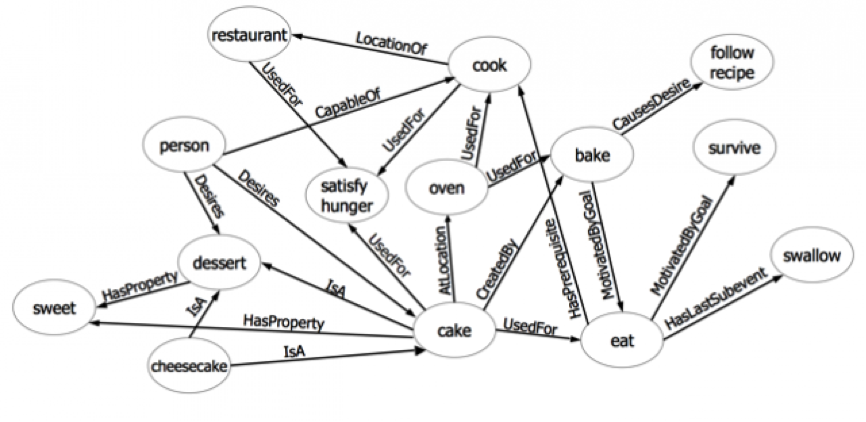
\includegraphics[width=\linewidth]{graph.png}
}
\caption{ConceptNet concept graph}
\label{graph}
\end{figure}


{\large Divisi}
is a library for reasoning by analogy and association over semantic networks, including common sense knowledge.
Divisi uses a sparse higher-order SVD can help find related concepts, features, and relation types in any knowledge base that can be represented as a semantic network. By including common sense knowledge from ConceptNet, the results can include relationships not expressed in the original data but related by common sense.


\section{Evaluation}
It is rather hard to evaluate recommender system, and even so with common sense knowledge because there is no
common criterions to evaluate common sense. However, since we haven't found the state of the art recommender engine
using common sense for gift recommendation, we have conducted a couple surveys and user studies to evaluate the accuracy
of our recommender system.

Based on time constraints, we conducted a usability test and two surveys with five National Taiwan University graduate students and alumnae.
The results of the surveys and the usability test are listed below.

\begin{table*}[ht]
\caption{Usability test results}
\centering
\begin{tabular}{| p{5cm} | c | c | c | c | c |}
\hline
Question & Subject 1 & Subject 2 & Subject 3 & Subject 4 & Subject 5 \\
\hline
Was the UI easy to use? & 3 & 4 & 3 & 3 & 4 \\
\hline
Did the options cover all my considerations for gift recommendation? & 3 & 4 & 3 & 4 & 3 \\
\hline
Were the ideal gifts in the result list? & 4 & 4 & 3 & 4 & 4 \\
\hline
Were most of the recommendations realistic? & 5 & 3 & 3 & 5 & 4 \\
\hline
Was the price checking feature helpful? & 4 & 5 & 5 & 5 & 4 \\
\hline
Will you consider using our system for gift recommendation in the future? & 5 & 4 & 4 & 5 & 4 \\
\hline
\end{tabular}
\label{table:usetest}
\end{table*}

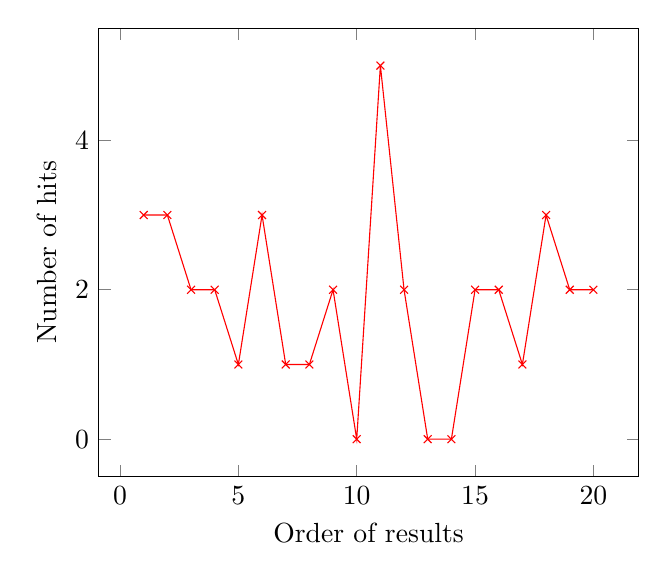
\begin{tikzpicture}
    \begin{axis}[xlabel=Order of results, ylabel=Number of hits]
    \addplot[color=red,mark=x] coordinates {(1,3) (2,3) (3,2) (4,2) (5,1) (6,3) (7,1) (8,1) (9,2) (10,0) (11,5) (12,2) (13,0) (14,0) (15,2) (16,2) (17,1) (18,3) (19,2) (20,2)};
    \end{axis}
\end{tikzpicture}

According to the plot above, the distribution is pretty even through out the search results but some bumpy hills along. We define hit rate as the number of times the tester's desired gift is ``hit'' on the result list. The higher the number the better our system performs. To illustrate the result of our survey in terms of hit rate, the scatter plot below provides the representation for that.

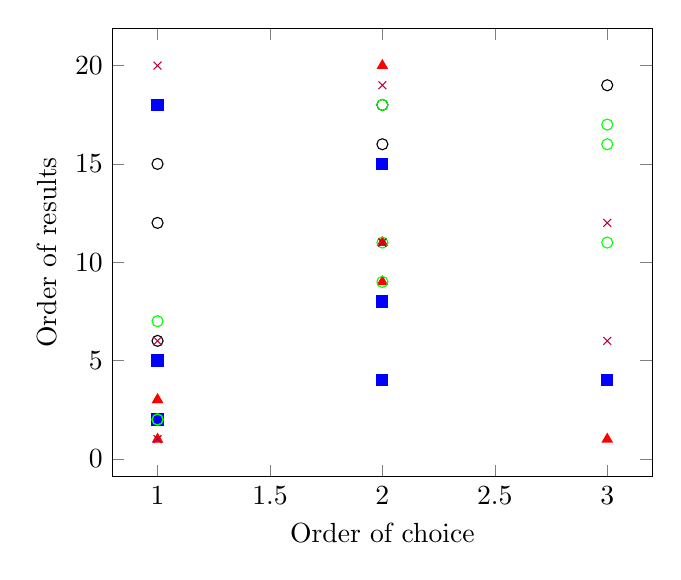
\begin{tikzpicture}
    \begin{axis}[
    xlabel=Order of choice,
    ylabel=Order of results,
    scatter/classes={
    a={mark=square*,blue},%
    b={mark=triangle*,red},%
    c={mark=o,draw=black},
    d={mark=o,draw=green},
    e={mark=x,draw=purple}
    }]
    \addplot[scatter,only marks,scatter src=explicit symbolic] 
    coordinates {
    (1, 5) [a]
    (2, 15) [a]
    (1, 18) [a]
    (2, 8) [a]
    (3, 4) [a]
    (1, 2) [a]
    (2, 4) [a]

    (1, 3) [b]
    (2, 20) [b]
    (1, 1) [b]
    (2, 9) [b]
    (1, 3) [b]
    (2, 11) [b]
    (3, 1) [b]

    (1, 15) [c]
    (1, 6) [c]
    (2, 18) [c]
    (3, 19) [c]
    (1, 12) [c]
    (2, 16) [c]

    (1, 7) [d]
    (2, 18) [d]
    (3, 16) [d]
    (1, 2) [d]
    (2, 11) [d]
    (3, 17) [d]
    (1, 2) [d]
    (2, 9) [d]
    (3, 11) [d]

    (1, 6) [e]
    (2, 11) [e]
    (3, 12) [e]
    (1, 1) [e]
    (2, 11) [e]
    (1, 20) [e]
    (2, 19) [e]
    (3, 6) [e]
    };
    \end{axis}
\end{tikzpicture}


\section{Conclusion}

Send gift is a cross culture social activity.  There are too many combinations in different occasions, different time and different situations.   Which gift should we pick?   Sometimes even expert might go wrong.   
As we mention in the beginning, our system is a good idea advisor rather than decision maker.   The assistant part let the system popular.   And the recommendation result does not have too many details. This kind of gift list help sender not only figure out what he/she really wants to send, but also let him/her think the part of surprise and intention.
The volunteer of our usability test gave a nice feedback of our system.   Most of the users answered that they will use our system if they plan to send a gift in the future.   This success not only attributed to good recommendation results, but also the great design of our UI.

\subsection{Future Work}

Gift recommendation is a new topic of this academic area.   There are no such ancestors to reference.   As a beginner of this domain, we can only evaluate our system by usability test. 

\subsubsection{Features}
Speaking to our system, the feature vector is build by us.   We merge a few people’s idea, then argue with each other, and finally come out the first version of feature table.
Although this table comes out a reasonable result, we still want to modify these data from the method like crowd voting, web mining and machine learning.   We believe that these methods will let feature table closer and closer to the truth value.

\subsubsection{Gift list}
On the other hand, our gift list has only 60 gifts.   We spent a long time browsing the internet, trying to summarize a list that can overlay the entire domain of the gift candidate and also not too much detail information.   We are going to build another page of GiftGiver which people can add new gift items on it.   If a particular gift owned more than 80% of “Is it suitable to be a gift item?” voting.   Then this gift might be added into our new gift list.

\subsubsection{Other information}
As you can see, the date part has not been used since our system build. In the future, we strongly hope that we can add locations or other useful information, and the commonsense part can be stronger when these information add in.


\newpage
\bibliographystyle{plain}
\bibliography{AAI}
\end{document}
